\section{Experiments}
\label{sec:experiments}

\paragraph{Baselines.}
\emph{Nearest ancestor} assigns each target to the closest ancestor.
\emph{Radial expansion} scales ancestor positions about the colony centroid by $\sqrt{N_b/N_a}$ before nearest assignment, \emph{radial sector} picks the ancestor in the most similar direction from it, and \emph{translation} aligns centroids.
\emph{Darcy} advects ancestors through the growth-pressure field of \cref{sec:darcy}, \emph{optical flow} along pretrained RAFT~\cite{teed2020raft} flow between the two images (chosen on M0--M2).
\emph{Unbalanced OT} (as in Waddington-OT~\cite{schiebinger2019optimal}) transports ancestors of mass $N_b/N_a$ to targets with a KL-relaxed ancestor marginal; we report the best of six variants on M0--M2 (Supp.~F).
\emph{Non-rigid CPD}~\cite{myronenko2010cpd} moves ancestors, as Gaussian centroids, smoothly onto the targets, each joining its most probable ancestor.
\emph{Forward simulation} (FSA) runs \rodsim from the first snapshot for $H$ minutes, warps the rollouts onto the second and assigns each target to the ancestor whose simulated descendants are densest there.
\emph{Family-centre regression} is a gradient-boosted regressor of each ancestor's descendant-family centre from hand-crafted neighbourhood features and $H$, followed by nearest assignment; it was our strongest model before \ours.
\emph{Trackastra}~\cite{gallusser2024trackastra} is a recent transformer tracker; we run its \texttt{general\_2d} model on the two snapshots with images and \emph{ground-truth} masks (greedy or argmax decoding), and fine-tuned on M0/M1, per gap or over five gaps, whichever is better on M2; removing its rotation augmentation does not help (Supp.~F).

\paragraph{Implementation.}
\ours has $d{=}128$, $T{=}4$ and is trained with AdamW (learning rate $5{\times}10^{-4}$, one-cycle schedule) for 30k steps (80k for the full and Darcy-initialised models) on one GPU (2.9M parameters, 1.3M for the genealogy network; 0.6--3\,h per model on a shared H200; 90\,ms per dense window, 1\,s with the decoder).
Cross-dataset experiments use positions-only models, as shape features differ across datasets; Supp.~A gives all details.
CIs are paired bootstraps over windows; under a block bootstrap respecting window overlap, all 33/66-minute margins over Trackastra, the direct matcher and the regressor remain, but no undecoded single model is significantly better at 132 minutes (Supp.~I).

\begin{table}[t]
\centering\small
\setlength{\tabcolsep}{3.5pt}
\begin{adjustbox}{max width=\linewidth}
\begin{tabular}{lcccccc}
\toprule
& \multicolumn{3}{c}{All windows} & \multicolumn{3}{c}{Dense ($N_a{>}200$)} \\
\cmidrule(lr){2-4}\cmidrule(lr){5-7}
Method & 33 & 66 & 132 & 33 & 66 & 132 \\
\midrule
Nearest ancestor & .497 & .361 & .263 & .157 & .083 & .058 \\
Radial expansion & .547 & .458 & .342 & .249 & .154 & .056 \\
Darcy flow prior (ours) & .627 & .466 & .368 & .305 & .161 & .088 \\
Optical flow (RAFT~\cite{teed2020raft}) & .636 & .367 & .244 & .347 & .094 & .041 \\
Unbalanced OT~\cite{schiebinger2019optimal} & .555 & .473 & .353 & .257 & .159 & .056 \\
Non-rigid CPD~\cite{myronenko2010cpd} & .597 & .466 & .359 & .294 & .162 & .060 \\
Family-centre regression (GBDT) & .731 & .610 & .446 & .449 & .297 & .201 \\
Trackastra~\cite{gallusser2024trackastra}, argmax & .681 & .176 & .162 & .395 & .073 & .057 \\
Trackastra, fine-tuned$^\dagger$ & .892 & .716 & .488 & .788 & .507 & .230 \\
\ours, rot.\ aug. & .741 & .604 & .451 & .459 & .294 & .178 \\
\ours, no rot. & .853 & .653 & .447 & .717 & .443 & .247 \\
Direct matcher (\ours, fixed centre) & .856 & .684 & .456 & .706 & .429 & .207 \\
\ours, full & .957 & .780 & .473 & .907 & .598 & .267 \\
\ours, ensemble + decoder & \textbf{.977} & \textbf{.863} & \textbf{.517} & \textbf{.946} & \textbf{.703} & \textbf{.300} \\
\ours, ensemble + decoder, no annotation & .963 & .822 & .487 & .919 & .634 & .260 \\
\midrule
\textcolor{gray}{Oracle family partition} & .984 & .929 & .784 & .963 & .817 & .465 \\
\bottomrule
\end{tabular}
\end{adjustbox}
\caption{\textbf{In-domain results on OIAM M3/M4} (trained on M0--M2). Accuracy at gaps of 33/66/132 minutes. Trackastra receives images and ground-truth masks of both snapshots. $^\dagger$Fine-tuned on M0/M1 lineage, one model per gap or one over five gaps, whichever is better on M2 (per gap at 33/66, over gaps at 132 minutes; checkpoint and decoding also chosen on M2). M3/M4 were inspected during development (leave-one-movie-out: supplement). Direct matcher: the same network with the family centre frozen at its initial position. Rot.\ aug./no rot.: 30k steps, radial initialisation, with/without rotation augmentation; full: see text. Direct matcher and full: mean of 3 seeds (std $\le$0.016); ensemble rows average the seeds' probabilities; no annotation: both networks trained on self-labelled lineage of the unannotated M0--M2; oracle: ensemble; other learned rows: one seed.}
\label{tab:oiam}
\end{table}


\subsection{Long gaps break frame-to-frame tracking}
\cref{tab:oiam} shows that off-the-shelf Trackastra, given perfect masks, improves over nearest assignment at 33 minutes but falls below it at 66 and 132 minutes; fine-tuned it is the strongest baseline, yet \ours without any annotation beats it at 33 and 66 minutes, on all 30 dense windows, and matches it at 132. No OT or CPD variant exceeds 0.60/0.51/0.38 (Supp.~F), and pretrained optical flow helps only at 33 minutes.
The \emph{full} model (no rotation augmentation, which exploits OIAM's fixed chamber geometry; Darcy initialisation; consistency loss; 80k steps) lifts 33-minute accuracy from 0.74 to $0.957{\pm}0.005$ (three seeds); with rotations it is better at 132 minutes over all windows but not on dense ones (Supp.~C).
The moving family centre is what matters: with it frozen, the same network reaches 0.86/0.68/0.46, and neither 96 candidates, nor a supervised but unused centre, nor one refinement round closes the gap at 33 and 66 minutes (pre-registered; Supp.~B). The centre is a remedy for crowding: its margin grows from 0.02 in windows of at most 25 ancestors to 0.24 above 400 (33 minutes, post hoc), and on the small van Vliet colonies it adds only 0.003 (pre-registered, failed; Supp.~B).
Retrained leaving out each OIAM movie in turn, the full model averages 0.95/0.79/0.48 on the held-out movie, as on M3/M4 (pre-registered; Supp.~D).
At 132 minutes Trackastra trained over several gaps edges the full model over windows (0.49 \vs 0.47) but not weighted by cells (0.29 \vs 0.32). On dense windows true family centres lift the ensemble from 0.28 to 0.50, the true partition to 0.47, both to 0.90 (Supp.~R).
Trained from scratch on M0/M1 only, \ours overfits (0.72/0.55/0.39; Supp.~F).
Above 400 ancestors at 33 minutes, nearest assignment, off-the-shelf and fine-tuned Trackastra and \ours are right for 13, 29, 74 and 89\% of targets (Supp.~G; a 66-minute window in \cref{fig:qualitative}).

\paragraph{How many snapshots are needed?}
\cref{fig:sparsity} composes links over equally spaced snapshots.
At 132 minutes, frame-to-frame linking with the fission prior reaches 0.96 with all 133 frames but 0.31 with 13, and Trackastra (true masks) 0.87 with 13; \ours reaches 0.90 with 5 snapshots and 0.99 with 13, which Trackastra needs 34 frames to match.
The self-labelled model (0.84 and 0.97) is close, and with every frame beats the linker that produced its labels (0.98 \vs 0.96).

\paragraph{Is the recovered lineage biologically usable?}
Longer cells divide sooner: over 33 minutes 79\% of the longest third of ancestors divide and 0.3\% of the shortest. \ours recovers this size control (71\% \vs 2.7\%; self-labelled 69\% \vs 3.9\%), nearest assignment erases it (34\% \vs 21\%). Decoded \ours halves decoded Trackastra's inflation of growth heterogeneity (Supp.~H).

\begin{figure}[t]
\centering
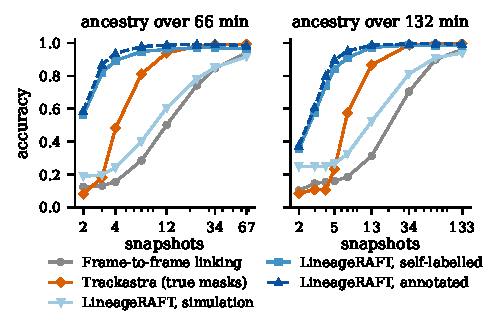
\includegraphics[width=\linewidth]{fig/sparsity.pdf}
\caption{\textbf{How many snapshots does lineage need?} Ancestry over 66 or 132 minutes on OIAM M3/M4 when the colony is imaged $n$ times at equal intervals and per-interval links are composed (32 random windows per gap, weighted by cells). Trackastra: off the shelf, true masks, argmax decoding (chosen on M2). Self-labelled: trained without any annotation.}
\label{fig:sparsity}
\end{figure}

\begin{figure*}[t]
\centering
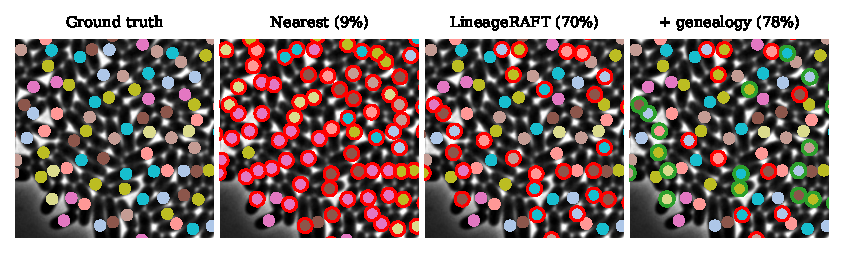
\includegraphics[width=0.74\linewidth]{fig/qualitative.pdf}
\caption{\textbf{A dense OIAM window at a 66-minute gap} (M4, 527 ancestors; crop of the target snapshot). Targets are coloured by their true (left) or predicted ancestor; red rings mark errors, green rings (right) errors of the network that the genealogy decoder corrects; percentages are accuracy over the whole window. Nearest assignment fails because cells moved more than the cell spacing; the genealogy fixes errors where neighbouring families interleave.}
\label{fig:qualitative}
\end{figure*}

\begin{table}[t]
\centering\small
\setlength{\tabcolsep}{3pt}
\begin{adjustbox}{max width=\linewidth}
\begin{tabular}{lccccccc}
\toprule
& \multicolumn{4}{c}{Baselines} & \multicolumn{2}{c}{\ours trained on} & Seq. \\
\cmidrule(lr){2-5}\cmidrule(lr){6-7}
Dataset & Nearest & Radial & Transl. & Other$^*$ & OIAM & \rodsim & wins \\
\midrule
FAST & .596 & .608 & .591 & .618$^{\mathrm{o}}$ & .615 & \textbf{.709} & 7/7 \\
recA & .452 & .470 & .462 & .481$^{\mathrm{o}}$ & .474 & \textbf{.560} & 9/9 \\
rpsM & .425 & .455 & .447 & .464$^{\mathrm{o}}$ & .465 & \textbf{.564} & 9/9 \\
OIAM & .374 & .449 & .345 & .487$^{\mathrm{d}}$ & .498 & \textbf{.520} & 2/2 \\
T98G & .889 & .896 & .898 & \textbf{.941}$^{\mathrm{o}}$ & .814 & .877 & 0/1 \\
LFCT & \textbf{.930} & .868 & .868 & .926$^{\mathrm{o}}$ & .793 & .894 & 0/1 \\
\bottomrule
\end{tabular}
\end{adjustbox}
\caption{\textbf{Zero-shot transfer.} Accuracy averaged over the three gaps of each dataset. Except for the OIAM-trained model on OIAM, no model saw labels from these datasets; the \rodsim model saw no real data at all. $^*$Best per dataset, in hindsight, of OT (o; three settings), CPD (c), Darcy advection (d) and \rodsim forward simulation (f), all fixed on OIAM M0--M2. \ours uses positions only. Last column: sequences on which \rodsim-trained \ours beats the best of all ten baselines (the columns, radial sector and the six behind Other; mean over gaps). \rodsim-trained: mean of three training seeds (per window); OIAM-trained: one seed, three movies, with rotation augmentation.}
\label{tab:external}
\end{table}


\subsection{Learning from simulation alone}
\cref{tab:external} evaluates positions-only \ours on datasets it was never trained on.
The model trained on OIAM M0--M2 barely improves on geometric baselines elsewhere and is worse on the human-cell datasets: it has learned the geometry of one experiment.
The model trained only on \rodsim is the best method on every bacterial dataset, by 3--10 points over the best baseline (three-seed mean), and wins on all 27 bacterial sequences; on FAST, Trackastra with images and true masks reaches 0.63 (pre-registered; Supp.~F).
The transfer is the simulator's: the direct matcher trained on the same simulations does as well (FAST/recA/rpsM/OIAM 0.71/0.57/0.58/0.50 \vs 0.71/0.56/0.56/0.52; pre-registered, Supp.~F). External windows hold 4--6 ancestors, where even in-domain the centre adds 0.01; on crowded OIAM windows the \rodsim-trained centre adds 0.02 (in-domain 0.19); forward simulation with true shapes beats it there (Supp.~Q), and simulating crowded colonies does not help (Supp.~R).
These datasets were seen while the simulator was designed (\cref{sec:sim}), so the clean zero-shot evidence is the blind test of \cref{tab:blind4}.
On the sparse human-cell datasets a baseline is best.


\begin{table}[t]
\centering\small
\setlength{\tabcolsep}{3pt}
\begin{adjustbox}{max width=\linewidth}
\begin{tabular}{llcccccc}
\toprule
 & Lineage & \multicolumn{3}{c}{All windows} & \multicolumn{3}{c}{Dense ($>$200)} \\
\cmidrule(lr){3-5}\cmidrule(lr){6-8}
Training & labels & 33 & 66 & 132 & 33 & 66 & 132 \\
\midrule
\multicolumn{8}{l}{\emph{Positions only, seed 0}} \\
\rodsim only & -- & .665 & .516 & .393 & .340 & .198 & .097 \\
\quad + fine-tune, true lineage & M0--M2 & .719 & .556 & .418 & .458 & .292 & .182 \\
\quad + fine-tune, self-labelled & none & .715 & .564 & .418 & .454 & .292 & .180 \\
\multicolumn{8}{l}{\emph{Full model (shape, Darcy), mean of three seeds}} \\
True lineage & M0--M2 & .957 & .780 & .473 & .907 & .598 & .267 \\
Self-labelled & none & .935 & .733 & .452 & .865 & .533 & .244 \\
\quad without consistency term (post hoc) & none & .940 & .759 & .456 & .877 & .577 & .258 \\
\bottomrule
\end{tabular}
\end{adjustbox}
\caption{\textbf{Self-labelling replaces lineage annotation} (OIAM M3/M4, accuracy, argmax). Self-labelled models are trained on lineage obtained by chaining one-frame links through the \emph{unannotated} M0--M2 time-lapses (\cref{sec:selflabel}); fine-tuning runs 6k steps from the \rodsim model, full models 80k steps from scratch (seed std $\le$0.013).}
\label{tab:selflabel}
\end{table}


\subsection{Self-labelling replaces lineage annotation}
Chaining one-frame links (\cref{sec:selflabel}) through the unannotated OIAM training movies recovers the true ancestor of 0.88--0.98 of cells at horizons of 33 to 240 minutes (Supp.~M).
Without the fission prior's daughter slots, links at divisions are wrong 30\% of the time instead of 4\% (pseudo-lineage at 132 minutes: 0.57 \vs 0.92).
\cref{tab:selflabel} trains on this pseudo-lineage instead of the annotation.
Fine-tuning the \rodsim model on it gains as much as on true lineage, and the full model trained from scratch on it comes within 0.02--0.05 of the annotated one over all windows (three seeds; \cref{tab:selflabel}); self-labelling costs the direct matcher only 0.01, yet self-labelled \ours beats the direct matcher trained on true lineage at 33/66 minutes (+0.08/+0.05; pre-registered, Supp.~M).
Self-labelling the genealogy network too (AP within 0.02; Supp.~K) removes annotation from every step: decoded ensembles reach 0.963/0.822/0.487 (fixed beforehand) \vs 0.977/0.863/0.517 (\cref{tab:oiam}).

\begin{table}[t]
\centering\small
\setlength{\tabcolsep}{4pt}
\begin{adjustbox}{max width=\linewidth}
\begin{tabular}{lcccccccc}
\toprule
Subset & $n$ & Best geom. & Best other & \rodsim & + Hung. & + boot. & \multicolumn{2}{c}{wins} \\
\cmidrule(lr){8-9}
 & & & & & & & \rodsim & boot. \\
\midrule
trpL & 10 & .574 & .591 & .674 & .598 & \textbf{.711} & 10/10 & 10/10 \\
metA & 9 & .497 & .517 & .636 & .542 & \textbf{.668} & 9/9 & 9/9 \\
pheA & 9 & .520 & .545 & .667 & .588 & \textbf{.714} & 9/9 & 9/9 \\
\bottomrule
\end{tabular}
\end{adjustbox}
\caption{\textbf{Pre-registered blind test} on three \emph{E.~coli} subsets of~\cite{vanvliet2018spatially} in minimal medium, never downloaded before the protocol was fixed (accuracy: mean over colonies of the mean over 30/60/120-minute gaps; run once). Best geom.: of nearest, translation, radial expansion and radial sector; best other: of exact and unbalanced OT (tuned on OIAM) and, added afterwards, radial-aligned OT, CPD, Darcy and forward simulation. Hung./boot.: \rodsim model fine-tuned on Hungarian-chained or bootstrapped pseudo-lineage of the other fold. Wins: colonies where \rodsim beats all ten baselines (also the six pre-registered), and where bootstrapping beats \rodsim.}
\label{tab:blind4}
\end{table}


\subsection{Pre-registered blind tests}
On unseen data we fixed each protocol, hypotheses included, before running it, and report every outcome (ledger: Supp.~O).
The first two failed instructively: on TrackRefiner~\cite{ahmadi2025trackrefiner} and TrackMate~\cite{anselmet2026trackmate} the \rodsim model won only on the 2 of 11 sequences showing a single colony (the others hold many microcolonies or are steady-state chambers), and on static \emph{B.~subtilis} spores~\cite{kunzmann2026bsub} nearest assignment is best.
Per-colony processing (post hoc) and self-labelling within each source (fixed beforehand) recover much of this, budding yeast~\cite{zelic2026lyn} included (Supp.~N).

A last test, with these procedures fixed, used three unused subsets of~\cite{vanvliet2018spatially}: 28 \emph{E.~coli} microcolonies in minimal medium from the lab and pipeline of recA/rpsM (\cref{tab:blind4}).
All four hypotheses hold on all three subsets: zero-shot, the \rodsim model beats every baseline on all 28 colonies, by 0.10 on average (95\% CI 0.09--0.11), and bootstrapped self-labelling from the other fold raises it further on all 28, whereas positions-only Hungarian self-labels lower it.



\begin{table}[t]
\centering\small
\setlength{\tabcolsep}{4pt}
\begin{adjustbox}{max width=\linewidth}
\begin{tabular}{llccc}
\toprule
Training data & Input & 33 & 66 & 132 \\
\midrule
& Base rate & .057 & .093 & .185 \\
OIAM M0--M2 & Geometry & .764 & .686 & .540 \\
OIAM M0--M2 & Image + geometry & .970 & .911 & .701 \\
\rodsim & Geometry & .088 & .119 & .201 \\
\rodsim & Image + geometry & .116 & .226 & .360 \\
\rodsim + division modes & Geometry & .490 & .491 & .460 \\
\rodsim + division modes & Image + geometry & .534 & .502 & .465 \\
\bottomrule
\end{tabular}
\end{adjustbox}
\caption{\textbf{Genealogy is visible in one snapshot.} Average precision for ``same ancestor $H$ minutes ago'' over 8-nearest-neighbour pairs in single OIAM M3/M4 frames. \rodsim rows use no real label; division-modes rows also render lineage (inherited intensity, septum constriction; alone: AP .110/.166/.219).}
\label{tab:genealogy}
\end{table}


\subsection{Genealogy from a single snapshot}
A single image carries much of the family structure that geometry lacks (\cref{tab:genealogy}).
At 33 minutes, where the positive pairs are mostly sisters from the last division, the image model reaches 0.97 AP against 0.76 for geometry and a 6\% base rate; even at 132 minutes it reaches 0.70 against 0.54.
Trained on \rodsim, it transfers only once division modes are randomised (V-snapping~\cite{messelink2021single}; added after inspecting OIAM M3), and then mostly through geometry (AP 0.53/0.50/0.47; 0.49/0.49/0.46 without the image).
In the Potts decoder ($\beta{=}2$, fixed), the image affinities improve every base model at every gap; the full model gains 0.034 at 66 minutes, the three-seed ensemble 0.057 (single models are overconfident; Supp.~I).
The decoder also lifts fine-tuned Trackastra at 33/66 minutes, yet decoded \ours stays ahead (pre-registered; Supp.~I). Non-local partitioners, a fission prior on family size and ancestors competing inside refinement leave 132-minute accuracy unchanged (the last helps dense windows; Supp.~I, R).


\subsection{Robustness to detection errors}
With 10\% of cells missed, merged or hallucinated, \ours is still 90--91\% correct at 33 minutes (nearest: 50\%).
With untuned Cellpose-SAM~\cite{pachitariu2025cellposesam} masks, \ours reaches 0.92/0.73/0.44; Omnipose~\cite{cutler2022omnipose} adds debris to sparse frames (0.74/0.50/0.29; Supp.~L).

\subsection{Limitations}
End-to-end results cover two segmenters on one dataset; synthetic detection errors ignore image content.
Trained from scratch on two annotated movies, \ours trails fine-tuned Trackastra (0.72 \vs 0.89 at 33 minutes; Supp.~F). OIAM's five movies are one experiment (the only public crowded lineage data we found), and the zero-shot advantage vanishes on fields of many tiny colonies or steady-state chambers.
Self-labelling needs a dense time-lapse per condition and inherits fast-motion linking errors (TrackRefiner).
